\documentclass[10pt]{article}
\usepackage[a4paper,landscape,margin=0.72in]{geometry}
\usepackage[T1]{fontenc}
\usepackage{lmodern,amsmath,amssymb,graphicx,hyperref}
\title{First all-closed-point divisor construction gate}
\author{Bounded formal API investigation and exact arithmetic diagnostic}
\date{28 October 2026}
\begin{document}
\maketitle
\noindent This packet adds no Lean theorem, global divisor, Picard-class result, experiment, or cost ratio. It records the exact first type-level gate and a reproducible finite-field input whose support is nonrational.

\section*{Pinned API and missing hypothesis}
Pinned Mathlib \texttt{AlgebraicGeometry/FunctionField.lean} defines the generic stalk of an irreducible scheme. Its \texttt{Field} instance and injective germ map require \texttt{IsIntegral X}. The actual weighted-$\operatorname{Proj}$ study has a checked two-open cover, affine domain, and smooth/proper structure map under their stated hypotheses, but no checked \texttt{IsIntegral} instance for the whole curve. Thus the source expression $n/B-Y$ is not yet an element of the actual scheme's function field in the project. The pinned height-one valuation finite-support API requires a Dedekind domain; no such instance or closed-point identification is checked for the affine chart.

\section*{Exact nonrational support diagnostic}
Over $\mathbf F_3$, set
\[
u_1=X^2+1,\quad u_2=X^2+X+2,\quad v_1=v_2=0,\quad
f=u_1u_2(X+2)=X^5+2X^3+X^2+X+1.
\]
Both quadratics have no $\mathbf F_3$ root: their value vectors at $0,1,2$ are $(1,2,2)$ and $(2,1,2)$. Exact polynomial arithmetic gives $\gcd(f,f')=1$, so $f$ is squarefree. Both valid Mumford congruences hold, the common 2+2 determinant is $B=1$, and $n=0$, $U=2X+1$ obey $n^2-u_1u_2U=B^2f$. Each quadratic support gives a degree-two closed point with residue field $\mathbf F_3[X]/(u_i)$; neither has an $\mathbf F_3$-rational support point. The committed stdlib checker reproduces the polynomial arithmetic. The closed-point quotient interpretation is a mathematical inference here, not a kernel-checked Lean theorem.

\section*{Next formal steps}
Prove the whole curve integral; map the source function from an affine chart into its generic stalk; construct a finitely supported order map over every closed point (including degree-two supports); specialize the infinity valuation; then state and prove its principal divisor. A scratch Lean probe was stopped after four minutes without compiler output. No compiler or axiom success is claimed for this packet. Exact scopes and source declarations are in the Markdown and CSV.

\clearpage
\section*{Dependencies}
\begin{center}
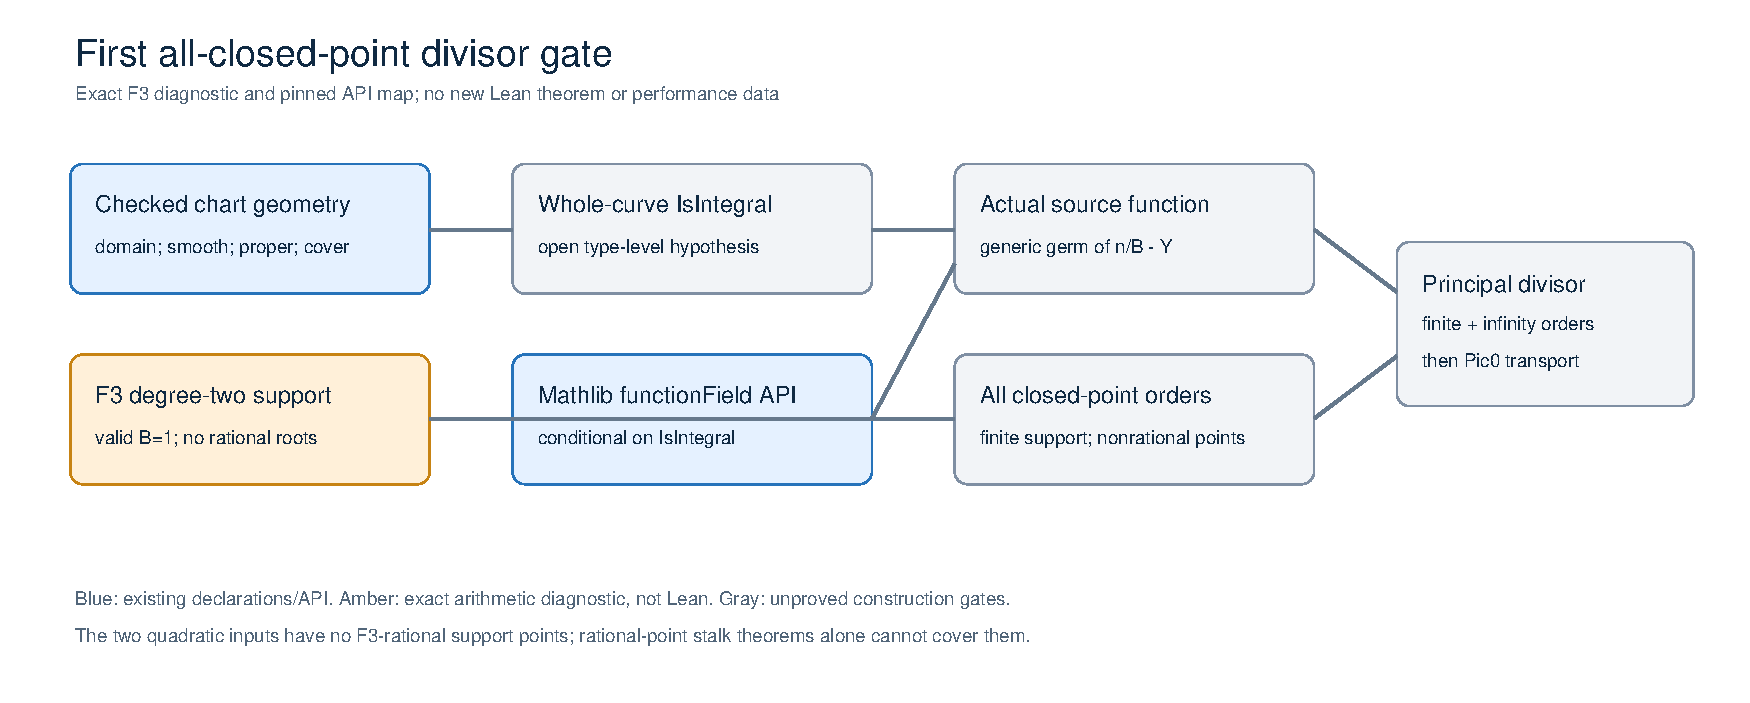
\includegraphics[width=0.96\textwidth,height=0.78\textheight,keepaspectratio]{function-field-gate-figure.pdf}
\end{center}
\noindent Blue: checked API/declarations; amber: exact arithmetic diagnostic; gray: open formal construction. Arrows are proof dependencies, not performance measurements.
\end{document}
